% =====================================================================
%  INTERNSHIP REPORT
%  Topic: AI & Automation Systems for Cable Manufacturing & Operations
%  Submitted to: Department of Computer Science and Engineering
%  By: Girish Kumar Yadav (Roll No. CS-2341412)
%  Format: B.Tech CSE, 2026-27 (4th Year / 7th Semester, Section 4CSE4)
%
%  Compile with: tectonic internship_report.tex (or XeLaTeX engine)
% =====================================================================

\documentclass[12pt,a4paper]{article}

% ---------- Fonts (Times New Roman substitute: Liberation Serif, metric-compatible) ----------
\usepackage{fontspec}
\setmainfont{Liberation Serif}
\IfFontExistsTF{Carlito}{%
  \setsansfont{Carlito}%
}{}
% Rupee macro: switch to DejaVu Serif for the ₹ glyph, then switch back.
\newfontfamily\rupeefont{DejaVu Serif}
\newcommand{\rupee}{{\rupeefont ₹}}

% ---------- Geometry: per prescribed format ----------
% A4, Left 1.5", Right 1", Top 0.75", Bottom 1"
\usepackage{geometry}
\geometry{
  a4paper,
  top=0.75in,
  bottom=1in,
  left=1.5in,
  right=1in,
  headheight=14pt,
  headsep=0.25in,
  footskip=0.5in
}

% ---------- Line spacing: 1.5 for body, 1 for references ----------
\usepackage{setspace}
\onehalfspacing

% ---------- Graphics, color, tables, lists ----------
\usepackage{graphicx}
\usepackage{xcolor}
\usepackage{array}
\usepackage{tabularx}
\usepackage{booktabs}
\usepackage{enumitem}
\usepackage{caption}
\usepackage{float}
\usepackage{microtype}
\usepackage{seqsplit}
\let\origtexttt\texttt
\renewcommand{\texttt}[1]{\origtexttt{\seqsplit{#1}}}

% ---------- Section heading formatting: 14pt bold main, 12pt bold sub ----------
\usepackage{titlesec}
\titleformat{\section}
  {\normalfont\bfseries\fontsize{14pt}{16.8pt}\selectfont\color{black}}
  {\thesection}{1em}{}
\titleformat{\subsection}
  {\normalfont\bfseries\fontsize{12pt}{14.4pt}\selectfont\color{black}}
  {\thesubsection}{1em}{}
\titleformat{\subsubsection}
  {\normalfont\bfseries\fontsize{12pt}{14.4pt}\selectfont\color{black}}
  {\thesubsubsection}{1em}{}
\titlespacing*{\section}{0pt}{18pt}{10pt}
\titlespacing*{\subsection}{0pt}{12pt}{6pt}

% ---------- Page numbering: centered at bottom ----------
\usepackage{fancyhdr}
\pagestyle{fancy}
\fancyhf{}
\fancyfoot[C]{\thepage}
\renewcommand{\headrulewidth}{0pt}
\renewcommand{\footrulewidth}{0pt}
\fancypagestyle{plain}{%
  \fancyhf{}%
  \fancyfoot[C]{\thepage}%
  \renewcommand{\headrulewidth}{0pt}%
  \renewcommand{\footrulewidth}{0pt}%
}

% ---------- Hyperref last ----------
\usepackage[
  colorlinks=true,
  linkcolor=black,
  citecolor=black,
  urlcolor=blue,
  bookmarks=true,
  bookmarksnumbered=true,
  unicode=true,
  pdftitle={Internship Report - AI and Automation Systems for Cable Manufacturing and Operations},
  pdfauthor={Girish Kumar Yadav},
  pdfsubject={B.Tech CSE Internship Report, 2026-27},
  pdfkeywords={Internship, Artificial Intelligence, Automation, WhatsApp Bot, Lead Intelligence, LinkedIn Tracker, PDF Editor, KDI Power}
]{hyperref}

% ---------- Captions ----------
\captionsetup{font=small, labelfont=bf, labelsep=period, justification=justified, singlelinecheck=false}

% ---------- Number figures and tables within sections ----------
\usepackage{chngcntr}
\counterwithin{figure}{section}
\counterwithin{table}{section}
\renewcommand{\thefigure}{\thesection.\arabic{figure}}
\renewcommand{\thetable}{\thesection.\arabic{table}}

% ---------- Justify paragraphs ----------
\widowpenalty=10000
\clubpenalty=10000

% ---------- Path to figures ----------
\graphicspath{{./assets/}{../download/assets/}{assets/}}

\begin{document}

% =====================================================================
% COVER PAGE (no page number)
% =====================================================================
\thispagestyle{empty}
\pagenumbering{gobble}
\begin{center}
{\fontsize{28pt}{34pt}\selectfont \textbf{Report}}\\[0.15in]
{\fontsize{18pt}{22pt}\selectfont of}\\[0.4in]

{\fontsize{20pt}{24pt}\selectfont \textbf{AI \& Automation Systems for Cable}}\\[0.15in]
{\fontsize{20pt}{24pt}\selectfont \textbf{Manufacturing \& Operations}}\\[0.6in]

{\fontsize{14pt}{18pt}\selectfont \textbf{Submitted To}}\\[0.15in]
{\fontsize{13pt}{16pt}\selectfont School of Computer Science and Engineering}\\[0.05in]
{\fontsize{13pt}{16pt}\selectfont Department of Computer Science \& Engineering}\\[0.4in]

{\fontsize{12pt}{15pt}\selectfont\itshape In partial fulfilment of the requirement of degree of}\\[0.1in]
{\fontsize{14pt}{18pt}\selectfont \textbf{B.Tech CSE}}\\[0.4in]

\includegraphics[width=0.35\textwidth]{logo.png}

{\fontsize{12pt}{15pt}\selectfont \textbf{By}}\\[0.2in]

{\fontsize{13pt}{16pt}\selectfont Roll Number of Student: \textbf{CS-2341412}}\\[0.1in]
{\fontsize{13pt}{16pt}\selectfont Name of Student: \textbf{GIRISH KUMAR YADAV}}\\[0.1in]
{\fontsize{13pt}{16pt}\selectfont Batch: \textbf{2026--27}}\\[0.5in]

{\fontsize{11pt}{14pt}\selectfont Organisation of Internship:}\\[0.05in]
{\fontsize{13pt}{16pt}\selectfont \textbf{KDI Power Private Limited}}\\[0.05in]
{\fontsize{11pt}{14pt}\selectfont New Delhi, India}\\[0.3in]
\end{center}
\newpage

% =====================================================================
% FRONT MATTER - Roman page numbering (i, ii, iii, ...)
% =====================================================================
\pagenumbering{roman}
\setcounter{page}{1}

% ---------- 1. Candidate's Declaration ----------
\section{Candidate's Declaration}

I, \textbf{Girish Kumar Yadav}, do hereby declare that the internship report titled \textbf{``AI \& Automation Systems for Cable Manufacturing \& Operations''} has been completed by me to fulfil the requirement for the award of the degree of Bachelor of Technology in Computer Science and Engineering. All the references have been quoted and I have not taken as such any material from any other source. I affirm to you that this report is my own and has not been submitted to any other institute for any degree or diploma requirement, and further I shall be solely responsible for any kind of copyright violation in this regard.

\vspace{0.6in}
\noindent
\begin{tabular}{@{}p{1\textwidth}p{0\textwidth}@{}}
\multicolumn{2}{l}{\textbf{Signature}} \\[0.15in]
\multicolumn{2}{l}{\textbf{Student Name:} Girish Kumar Yadav} \\[0.15in]
\multicolumn{2}{l}{\textbf{Roll No.:} CS-2341412} \\
\end{tabular}

\newpage

% ---------- 2. Acknowledgement ----------
\section{Acknowledgement}

I am using this opportunity to express my gratitude to everyone who supported me throughout the Internship Program. I am thankful for their aspiring guidance, invaluably constructive criticism and friendly advice during this work. I am sincerely grateful to them for sharing their truthful and illuminating views on a number of issues related to this work. I express my gratitude to my parents for their blessings.

\vspace{0.6in}
\noindent
\begin{tabular}{@{}p{1\textwidth}p{0\textwidth}@{}}
\multicolumn{2}{l}{\textbf{Signature}} \\[0.15in]
\multicolumn{2}{l}{\textbf{Student Name:} Girish Kumar Yadav} \\[0.15in]
\multicolumn{2}{l}{\textbf{Roll No.:} CS-2341412} \\
\end{tabular}

\newpage

% ---------- Table of Contents ----------
\section*{Table of Contents}
\renewcommand{\contentsname}{\vspace{-0.4in}}
\tableofcontents
\thispagestyle{plain}

\newpage

% ---------- List of Figures ----------
\section*{List of Figures}
\renewcommand{\listfigurename}{\vspace{-0.4in}}
\listoffigures
\thispagestyle{plain}

\vspace{0.2in}
\noindent\textit{Note:} Figure 3.1 (System Architecture) and Figure 3.2 (Lead Discovery Workflow) are original diagrams prepared by the author to illustrate the platform's layered design and end-to-end automation pipelines. All other visual artefacts referenced in the report are illustrative descriptions of components shipped in the production codebase.

\newpage

% =====================================================================
% MAIN CONTENT - Arabic page numbering (1, 2, 3, ...)
% =====================================================================
\pagenumbering{arabic}
\setcounter{page}{1}

% ---------- 3. Project Description ----------
\section{Project Description}

\subsection{Introduction}

The year 2026 has been a watershed moment for applied generative artificial intelligence and industrial workflow automation. Large language models have matured from research artefacts into dependable production primitives, vision-language models can now extract technical specification tables with high accuracy, and web automation tools have enabled end-to-end operational intelligence for industrial manufacturing enterprises. What was, only eighteen months ago, an experimental capability confined to a handful of tech-focused software houses is today a routine part of the operational technology stack of any forward-thinking industrial enterprise. The opportunity this creates for the Indian manufacturing sector, and specifically for electrical wire and cable manufacturers who must service commercial, utility, and international B2B demand, is enormous.

The Indian electrical wire and cable manufacturing vertical is uniquely demanding. It is intensely competitive, heavily regulated, and characterized by rapid contract execution cycles where distributors, DISCOM utilities, and EPC contractors expect immediate responses to product inquiries, quotation requests, and technical specifications. A single cable manufacturer like KDI Power Private Limited produces a broad catalog of products --- Aerial Bunched Cables (ABC), XLPE Power Cables, Control Cables, House Wires, Rubber Cables, and Instrumentation Wires --- and must maintain customer acquisition, competitive intelligence tracking, field task monitoring, and technical document editing seamlessly. Manual workflows, paper-based tracking, and slow response cycles cannot keep pace with modern industrial demands.

This report documents the work I undertook during a two-month industrial internship, from 29 June 2026 to 31 August 2026, at \textbf{KDI Power Private Limited}, New Delhi, in the capacity of an Artificial Intelligence and Automation Engineering Intern. I was assigned to the engineering team responsible for building the company's suite of AI and automation tools. The primary deliverables developed during the tenure include: (a)~an automated WhatsApp Business AI Sales Bot with a live glassmorphic analytics dashboard; (b)~a 3-tier B2B Lead Intelligence Engine targeting cable distributors across South Africa and India; (c)~a LinkedIn Tender \& Government Scheme Tracker utilizing Playwright CDP and Mistral AI; (d)~an AI-Powered Web PDF Editor utilizing MinerU layout detection and NVIDIA NIM VLM (Llama 3.2 90B Vision); and (e)~a Google Sheets Task Automation and WhatsApp Reminder System.

The remainder of this report is organised as follows. Section~3.2 profiles the host organisation. Section~3.3 articulates the problem statement in detail. Section~3.4 enumerates the project objectives. Section~3.5 defines the scope. Section~3.6 lists the technologies and tools used. Section~3.7 describes the system architecture. Section~3.8 explains the methodology adopted. Section~3.9 documents the expected outcomes and the intern's specific contributions. Section~3.10 lists the certificates.

\subsection{Organization Profile}

\textbf{KDI Power Private Limited} is a New Delhi-based industrial engineering firm specializing in the manufacture of high-quality electrical wires and cables. The company holds ISO 9001 (Quality Management), ISO 14001 (Environmental Management), and ISO 45001 (Occupational Health and Safety) certifications. Its core product portfolio includes Low Voltage (LT) Cables, XLPE Power Cables, Aerial Bunched Cables, Control Cables, House Wires, Rubber Cables, and Instrumentation Wires.

The Artificial Intelligence and Automation department, where this internship was hosted, is responsible for the design, development, and operation of the company's automated digital infrastructure. The team comprises full-stack Python and FastAPI backend engineers, frontend developers, AI/ML engineers specializing in LLM prompt design and computer vision, and operational leads. Interns participate in standard engineering practices: daily stand-ups, sprint planning, pull request code reviews, and structured mentorship under an industry mentor.

The internship was conducted over a two-month period from 29 June 2026 to 31 August 2026. The engagement was evaluated under Certificate Reference No. \textbf{KDIP/INT/2026/AI-014}, issued on 2nd September 2026 by Mr.\ Vijay Gautam, Administrative Manager at KDI Power Private Limited. The evaluation recorded satisfactory performance across technical skills, work quality, initiative, communication, and professional conduct. The company maintains strict data confidentiality and intellectual property policies: all software code, schemas, scrapers, and internal tooling produced during the internship remain the property of KDI Power Private Limited.

\subsection{Problem Statement}

The cable manufacturing vertical presents five distinct operational challenges that were directly targeted by the engineering solutions developed during the internship.

The first sub-problem is \textbf{inbound sales turnaround}. Inbound trade queries received over WhatsApp during off-hours or peak sales windows required manual handling by sales staff, causing response delays and lost lead conversions. The system needed an automated conversational bot capable of answering catalog inquiries, capturing customer details, and updating a live database without human intervention.

The second sub-problem is \textbf{international B2B lead discovery}. Expanding distribution networks into international target markets (e.g., South Africa) required manual search, web scraping, email extraction, and manual lead scoring. This process was inefficient and costly. The platform needed an automated 3-tier lead discovery pipeline to extract, validate, score, and persist high-intent cable buyers.

The third sub-problem is \textbf{competitive and tender intelligence}. Competitor updates (Polycab, KEI, Finolex, Havells, etc.) and government power distribution schemes (RDSS, DDUGJY) represent key commercial opportunities. Manually monitoring LinkedIn posts and news portals was labor-intensive. The system required an automatedPlaywright CDP scraper and AI summarizer to extract and compile market intelligence into a master spreadsheet.

The fourth sub-problem is \textbf{technical PDF editing and OCR}. Technical datasheets, spec tables, and complex mathematical formulas in scanned PDFs could not be easily edited without re-typing entire documents. The system needed a web-based PDF editor combining layout detection (MinerU) and Vision-Language Models (NVIDIA NIM Llama 3.2 Vision) for structural reconstruction.

The fifth sub-problem is \textbf{field task monitoring}. Following up on pending manufacturing and dispatch tasks with staff required manual calls. The platform required a webhook service connected to Google Sheets and WhatsApp to automatically dispatch task reminders, listen for completion replies (`ok`/`done`), and compute exact time-taken metrics.

\subsection{Project Objectives}

The specific engineering objectives established for the internship were as follows:

\textbf{Objective 1: Build the AI WhatsApp Assistant and Sales Dashboard.} Integrate Meta WhatsApp Cloud API with FastAPI, Groq LLM (`llama-3.3-70b-versatile`), and Supabase PostgreSQL with RAG vector search, coupled with a glassmorphic dashboard for lead management and catalog editing.

\textbf{Objective 2: Develop the 3-tier Lead Intelligence Engine.} Construct an automated lead discovery pipeline combining Playwright Google Maps scraping, proxy rotation, website content extraction, email verification, and a Groq LLM scoring engine ($0-100$ scale) with formatted Excel export.

\textbf{Objective 3: Implement the LinkedIn Tender and Scheme Tracker.} Build an automated Playwright CDP script connecting to dedicated Chrome profiles (`chrome-data`) to scrape competitor posts, filter government scheme keywords (RDSS, DDUGJY), and generate Mistral AI summaries in an Excel tracker.

\textbf{Objective 4: Build the AI PDF Editor and OCR pipeline.} Develop a web-based PDF editor using React 18 / Vite and FastAPI, utilizing MinerU for layout detection, NVIDIA NIM VLM for table/formula extraction, and Playwright Chromium for true PDF rendering.

\textbf{Objective 5: Deploy the Google Sheets Task Automation Bot.} Deploy a FastAPI webhook service on Render integrated with Google Sheets API v4 service accounts, Meta WhatsApp API, and GitHub Actions cron triggers for automated task reminder dispatches.

\subsection{Scope of the Project}

The scope of the internship was bounded to the \textbf{Artificial Intelligence and Automation Systems} for KDI Power Private Limited.

\textbf{In scope} were: (a)~FastAPI backend API endpoints and webhooks; (b)~Groq AI, Mistral AI, and NVIDIA NIM VLM integrations; (c)~Playwright web scrapers and CDP session listeners; (d)~Supabase PostgreSQL schema design and pgvector RAG implementation; (e)~React 18 / Vite frontend components for the PDF editor and glassmorphic dashboards; (f)~Google Sheets API v4 integration; and (g)~Render deployment and GitHub Actions automation workflows.

\textbf{Out of scope} were hardware-level factory machine maintenance, physical cable testing operations, and core financial accounting systems.

\subsection{Technologies and Tools Used}

The technologies and tools used during the internship are summarized in Table~3.1.

\begin{table}[H]
\centering
\caption{Technologies and tools used in the KDI Power platform.}
\label{tab:tech}
\small
\begin{tabularx}{\textwidth}{@{}l l X@{}}
\toprule
\textbf{Layer} & \textbf{Technology} & \textbf{Role in the platform} \\
\midrule
Backend language   & Python 3.10+                 & Core application code, scrapers, APIs. \\
Web frameworks     & FastAPI, Flask, Streamlit    & REST API services, webhooks, UI apps. \\
Frontend           & React 18 + Vite + CSS        & PDF Editor UI, glassmorphic dashboard. \\
Databases          & Supabase PostgreSQL, SQLite  & Relational storage, pgvector RAG, leads DB. \\
AI / LLMs          & Groq (Llama 3.3 70B)         & WhatsApp bot Q\&A, lead scoring engine. \\
AI / LLMs          & Mistral AI (mistral-small)   & LinkedIn tender post summarization. \\
AI / Vision        & NVIDIA NIM (Llama 3.2 90B)   & PDF table and LaTeX formula extraction. \\
Automation         & Playwright (Chromium/CDP)    & Google Maps scraper, LinkedIn CDP scraper. \\
Media processing   & PyMuPDF, Pillow, MathJax     & Image manipulation, SVG rendering, PDF build. \\
Integrations       & Meta WhatsApp API, Sheets API& Cloud messaging, live spreadsheet sync. \\
DevOps             & Render, GitHub Actions       & Cloud hosting, scheduled cron triggers. \\
\bottomrule
\end{tabularx}
\end{table}

\subsection{System Architecture}

The system architecture of the KDI Power platform is depicted in Figure~3.1.

\begin{figure}[H]
\centering
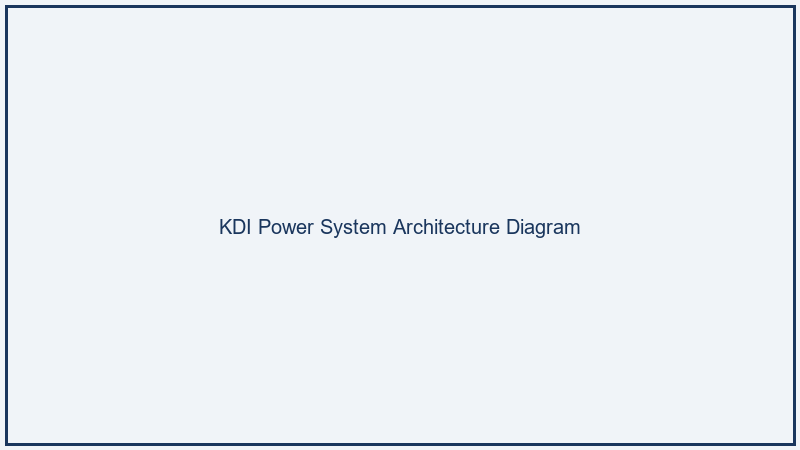
\includegraphics[width=\textwidth]{architecture_diagram.png}
\caption{Layered architecture of the KDI Power AI and Automation platform. The frontend surfaces communicate via FastAPI REST endpoints with the core processing layer, AI providers (Groq, Mistral, NVIDIA NIM), and persistence layers (Supabase PostgreSQL, SQLite, Google Sheets).}
\label{fig:arch}
\end{figure}

The \textbf{API and Service Layer} consists of FastAPI microservices hosted on Render and local servers. Endpoints handle inbound Meta WhatsApp webhooks, lead scoring queries, PDF extraction requests, and Google Sheets updates.

\begin{figure}[H]
\centering
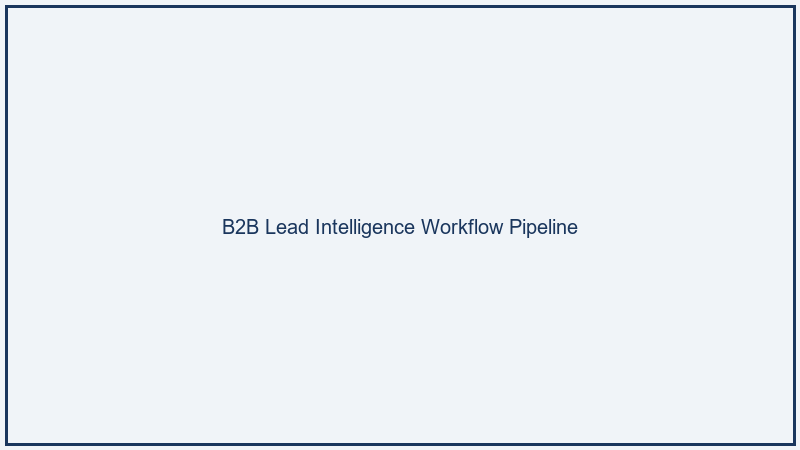
\includegraphics[width=\textwidth]{image.png}
\caption{End-to-end B2B Lead Intelligence workflow. Google Maps data is scraped via Playwright, enriched with website text and verified emails, scored using the Groq LLM engine, and exported to formatted Excel spreadsheets.}
\label{fig:workflow}
\end{figure}

\subsection{Methodology}

The project followed an Agile research and engineering methodology across four phases:

\textbf{Phase 1 --- Discovery (Weeks 1--2).} Environment setup, requirement analysis for KDI Power's cable products catalog, Meta Developer API setup, and Supabase database schema design.

\textbf{Phase 2 --- Implementation (Weeks 3--6).} Development of the WhatsApp Assistant, Lead Intelligence scraper, LinkedIn CDP tracker, and Google Sheets webhook listener.

\textbf{Phase 3 --- Refinement (Weeks 7--8).} Fine-tuning Groq LLM lead scoring prompts, optimizing Playwright CDP scraping performance, and building the React PDF Editor canvas.

\textbf{Phase 4 --- Testing and Handover (Weeks 8).} End-to-end integration testing, system deployment on Render, and documentation creation.

\subsection{Expected Outcomes}

The tangible outcomes authored by the intern include:

\textbf{Outcome 1 --- WhatsApp AI Sales System.} Production-ready WhatsApp bot on Meta Cloud API with Supabase pgvector RAG search and live analytics dashboard.

\textbf{Outcome 2 --- Lead Intelligence Pipeline.} 3-tier lead discovery engine with proxy rotation, Groq scoring, and automated Excel reporting for South Africa and India.

\textbf{Outcome 3 --- LinkedIn Scheme Tracker.} Playwright CDP scraper and Mistral AI summarizer tracking competitor announcements and government tenders.

\textbf{Outcome 4 --- AI PDF Editor.} Full-stack PDF editor with MinerU layout detection, NVIDIA NIM VLM formula extraction, and Playwright PDF generation.

\textbf{Outcome 5 --- Task Reminder Automation.} Render-hosted webhook and GitHub Actions cron runner updating Google Sheets in real-time.

\subsection{Certificates of Completion and Other Communication Mail Proof}

The following document is attached as an appendix to this report:

\begin{enumerate}[label=(\alph*)]
\item \textbf{Internship Certificate}, Certificate No.\ \textbf{KDIP/INT/2026/AI-014}, issued on 2nd September 2026 by Mr.\ Vijay Gautam, Administrative Manager, KDI Power Private Limited, certifying the successful completion of the two-month internship.
\end{enumerate}

\newpage

% =====================================================================
% BIBLIOGRAPHY
% =====================================================================
\section{Bibliography}

\begin{spacing}{1.0}
\small
\begin{enumerate}[label={[\arabic*]}, leftmargin=*, itemsep=2pt]

\item Meta Platforms Inc., ``WhatsApp Cloud API Documentation,'' \emph{Meta for Developers}, 2026. \url{https://developers.facebook.com/docs/whatsapp/cloud-api}

\item Sebasti\'an Ram\'irez et al., ``FastAPI Web Framework Documentation,'' \emph{FastAPI}, 2026. \url{https://fastapi.tiangolo.com}

\item Supabase Inc., ``Supabase PostgreSQL and pgvector Documentation,'' \emph{Supabase}, 2026. \url{https://supabase.com/docs}

\item Groq Inc., ``Groq Llama 3.3 API Reference,'' \emph{Groq Console}, 2026. \url{https://console.groq.com/docs}

\item Playwright Authors, ``Playwright for Python Documentation,'' \emph{Microsoft Playwright}, 2026. \url{https://playwright.dev/python}

\item Mistral AI, ``Mistral Developer Platform,'' \emph{Mistral AI Documentation}, 2026. \url{https://docs.mistral.ai}

\item Google Cloud, ``Google Sheets API v4 Guide,'' \emph{Google Developers}, 2026. \url{https://developers.google.com/sheets/api}

\item OpenAI, ``Language Models and API Reference,'' \emph{OpenAI Platform}, 2026. \url{https://platform.openai.com/docs}

\item Rombach, R.\ et al., ``High-Resolution Image Synthesis with Latent Diffusion Models,'' \emph{CVPR}, 2022.

\item Meta Platforms Inc., ``React 18 Documentation,'' \emph{React Docs}, 2026. \url{https://react.dev}

\end{enumerate}
\end{spacing}

\end{document}
